%*******************************************************************
%   Project Name: BracU Thesis Template
%   Prepared by: Ayesha Abed Library, Brac University
%   
%   "Predicting a T20 Cricket Match Result While The Match is in Progress", this thesis was 
%   submitted to BracU on 23 August, 2015 by Fahad Munir, Md. Kamrul Hasan, Sakib Ahmed, Sultan Md. Quraish
%   Authors have given full consent to use their thesis as a sample to develop a Thesis Template using LaTex 
%   PLEASE KEEP ALL FILES IN THEIR DESIGNATED FOLDERS
%*******************************************************************
% Project Structure:
% appendix: Contains “appendix.txt” files.
% bibliography: Contains “references.bib” file.
% chapters: Contains “chapter.txt” files. For every chapter, create separate “chapter_[1,2,3..].txt” files.
% core: This folder will contain following files:
%     declaration.txt
%     approval.txt
%     ethics_statement.txt
%     abstract.txt
%     dedication.txt
%     acknowledgement.txt
%     titlepage.txt
% images:Contains all images files. 
% main.txt
%     This is the main.txt file. All the packages and environment variable are declared in main.txt. All others .txt files are referred from this file.
%
% If you have any questions or concerns about the latex template, please feel free to visit Ayesha Abed Library.
%*******************************************************************

\documentclass[Times,12pt,oneside,openany,print,index]{report}
\usepackage[a4paper,width=150mm,top=25mm,bottom=25mm]{geometry}
\usepackage[english]{babel}
\usepackage[utf8]{inputenc}
\usepackage{csquotes} % Provides advanced facilities for in-line and display quotations
\usepackage{amsmath} % TO use mathematical equations 
\usepackage{float}
\pagestyle{plain} % Just a plain page number. For more http://www.emerson.emory.edu/services/latex/latex_129.html

\usepackage{graphicx} % to use the graphicx package
\graphicspath{/images} % Path to Image files 
\usepackage{caption} % To use caption with figure and images
\usepackage{array} % The array environment is used to make a table of information, with column alignment (left, center, or right) and optional vertical lines separating the columns

\usepackage[nottoc]{tocbibind} % The tocbibind package can be used to add the ToC and/or bibliography and/or the index etc., to the Table of Contents listing

\usepackage[normalem]{ulem} % The ulem package provides various types of underlining that can stretch between words and be broken across lines.

\usepackage{hyperref} % Provides LaTeX the ability to create hyperlinks within the document.
\hypersetup{
    colorlinks=true,
    linkcolor=black,
    filecolor=magenta,      
    urlcolor=black,
    citecolor=black,
}
\urlstyle{same}

\setlength{\parindent}{0em} % To control Indentation of paragraphs 

\usepackage{nomencl} % The nomenclature package can be used to generate and format a nomenclature using MakeIndex.
\renewcommand{\nompreamble}{The next list describes several symbols \& abbreviation that will be later used within the body of the document}
\makenomenclature

\usepackage[backend=biber,style=ieee,sorting=ynt]{biblatex} % for more plz click https://www.overleaf.com/learn/latex/Biblatex_citation_styles
\addbibresource{bibliography/references.bib} % Imports bibliography file

\let\cleardoublepage=\clearpage % removes unwanted doublepages

\begin{document}

\thispagestyle{empty} % removes page number from title page
\begin{titlepage}
\renewcommand*{\thepage}{Title} % Change page number in PDF

    \begin{center} 
        \vspace*{3cm} % For creating Vertical Blank Space
        
        {\fontsize{16pt}{22pt}\selectfont{Efficient LLM Distillation for Bangladesh Legal Context: A Smartphone-Compatible Retrieval-Augmented Generation Model}
        } % "fontsize{font size}{line space}\selectfont{}" command to override font size and line space for the Title
        
        \vspace{1.5cm}
        
        \text{by}
        
        \vspace{0.5cm}
        
        	Talha Ridwan\\
	        24341161\\
	        Mahadi Hasan Fahim\\
	        22301128\\
            Nadifa Zaman\\
	        22301126\\
	        MD. Nafis Kamal\\
	        22301031\\
	        Fariha Roushon Florin\\
                22201622

        \vspace{1.5cm}
        
        	A thesis submitted to the Department of Computer Science and Engineering\\
            in partial fulfillment of the requirements for the degree of\\
            B.Sc. in Computer Science and Engineering

        
        \vspace{2.5cm}
        
    		Department of Computer Science and Engineering\\
            Brac University\\
            June 2025.
        
        \vspace{3cm}
        
    		\copyright\ 2025. Brac University\\
            All rights reserved.
    
    \end{center}

\end{titlepage} % Add title page
\cleardoublepage

\pagenumbering{roman} % Roman numbers to be use all pages before Chapter 1

%*******************************************************************
% TOC = Table of Contents
% The hyperref makes Title page No. 1 entry in the TOC
% In order to properly link  all section in TOC "phantomsection" command used
%  see below link for details on "addcontentsline"
% http://www.emerson.emory.edu/services/latex/latex_162.html
% "input" command to add files
% "Ethics Statement" & "Dedication" page are Optional; you may omit this two page if you want
% Please do not change the order of listings in TOC
%*******************************************************************
\phantomsection
\addcontentsline{toc}{chapter}{Declaration}
% Following command is used to created grouped signature line for Four Authors
\newcommand*\wildcard[2][6cm]{\vspace{2cm}\parbox{#1}{\hrulefill\par#2}} 

% A "parbox{}{}" is a box whose contents are created in paragraph mode. 
% "hrulefill{} to chance thickness of underline"

\section*{Declaration}

It is hereby declared that

\begin{enumerate} % begin{enumerate} function to create numbered list
  \item The thesis submitted is my/our own original work while completing degree at Brac University.
  \item The thesis does not contain material previously published or written by a third party, except where this is appropriately cited through full and accurate referencing.
  \item The thesis does not contain material which has been accepted, or submitted, for any other degree or diploma at a university or other institution.
  \item We have acknowledged all main sources of help.
\end{enumerate}

\vspace{1cm}
\textbf{Student’s Full Name \& Signature:} % Testbf{} for Bold


\begingroup

    \begin{center}
    \begin{tabular}{p{5cm} p{5cm}}
    \begin{minipage}[t]{4.5cm}
            \centering
            
\includegraphics[width=0.6\linewidth]{images/sign_talha.jpg} \\
            \rule{4cm}{0.4pt} \\
            \vspace{0.1cm}
            Talha Ridwan \\
            24341161
        \end{minipage}
        
        \begin{minipage}[t]{4.5cm}
            \vspace{0.3cm}
            \centering
            
\includegraphics[width=0.6\linewidth]{images/sign_mahadi.jpg} \\
            \rule{4cm}{0.4pt} \\
            \vspace{0.1cm}
            Mahadi Hasan Fahim \\
            22301128
        \end{minipage}
        &
        \begin{minipage}[t]{4.5cm} 
            \centering
            
\includegraphics[width=0.6\linewidth]{images/sign_nafis.jpg} \\
            \rule{4cm}{0.4pt} \\
            \vspace{0.1cm}
            MD. Nafis Kamal \\
            22301031
        \end{minipage} \\
        \vspace{1cm} \\
        \begin{minipage}[t]{4.5cm}
            \centering
            
\includegraphics[width=0.6\linewidth]{images/sign_nadifa.jpg} \\
            \rule{4cm}{0.4pt} \\
            \vspace{0.1cm}
            Nadifa Zaman \\
            22301126
        \end{minipage}
        &
        \begin{minipage}[t]{4.5cm}
            \centering
            
\includegraphics[width=0.6\linewidth]{images/sign_fariha.jpg} \\
            \rule{4cm}{0.4pt} \\
            \vspace{0.1cm}
            Fariha Roushon Florin \\
            22201622
        \end{minipage}
    \end{tabular}
\end{center}

\endgroup



\pagebreak







\phantomsection
\addcontentsline{toc}{chapter}{Approval}
\section*{Approval}

The thesis/project titled “Efficient LLM Distillation for Bangladesh Legal Context: A Smartphone-Compatible Retrieval-Augmented Generation Model” submitted by 
\begin{enumerate}
  \item Talha Ridwan (24341161)
  \item Mahadi Hasan Fahim (22301128)
  \item MD. Nafis Kamal (22301031) 
  \item Nadifa Zaman (22301126)
  \item Fariha Roushon Florin (22201622)
\end{enumerate}

of Summer, 22 has been accepted as satisfactory in partial fulfillment of the requirement for the degree of B.Sc. in Computer Science in Spring 25. 

\vspace{0.5cm}
\textbf{Examining Committee:}

\vspace{1cm}

Supervisor:\\
(Member)
\begin{center}
    \hspace{7cm}
\includegraphics[width=0.2\linewidth]{images/sign_sadaat_sir.png} \\
    \hspace{7cm} \wildcard{\centerline{Saadat Rafid Ahmed} ~\\ \centerline{Lecturer}~\\ 
    \centerline{Department of Computer Science and Engineering}~\\ \centerline{BRAC University} } \hspace{1cm} 
\end{center}

Co-Supervisor:\\
(Member)
\begin{center}
    \hspace{7cm}
\includegraphics[width=0.2\linewidth]{images/sign_farig_sir.png} \\
    \hspace{7cm} \wildcard{\centerline{Dr. Farig Yousuf Sadeque} ~\\ \centerline{Associate Professor}~\\ \centerline{Department of Computer Science and Engineering}~\\ \centerline{BRAC University} } \hspace{1cm} 
\end{center}

\pagebreak
Thesis Coordinator:\\
(Member)
\begin{center}
    \hspace{7cm} \wildcard{\centerline{Dr. Md. Golam Rabiul Alam} ~\\ \centerline{Professor}~\\ \centerline{Department of Computer Science and Engineering}~\\ \centerline{BRAC University} } \hspace{1cm} 
\end{center}

Head of Department:\\
(Chair)
\begin{center}
    \hspace{7cm} \wildcard{\centerline{Dr. Sadia Hamid Kazi} ~\\ \centerline{Chairperson}~\\ \centerline{Department of Computer Science and Engineering }~\\ \centerline{BRAC University} } \hspace{1cm} 
\end{center}

\pagebreak

%\phantomsection
%\addcontentsline{toc}{chapter}{Ethics Statement}
%\section*{Ethics Statement (Optional)}
This is optional, if you don't have an ethics statement then omit this page
\pagebreak

\phantomsection
\addcontentsline{toc}{chapter}{Abstract}
\section*{Abstract}
Large Language Models (LLMs) are highly effective at  finding and generating information. Still they are difficult to use on devices with limited processing capacity like smartphones as they require a lot of computing power. This thesis focuses on creating a smaller and more efficient Retrieval-Augmented Generation (RAG) model. The model will be specifically designed to work with Bangladesh’s legal system. To make the model lighter and faster, we will use LLM distillation . This process removes the unnecessary parts of a large model while keeping its ability of finding and generating desired information from a specific domain. The goal is to reduce the model size to less than under a billion parameters. Our approach will make sure that the model works smoothly on personal devices like smartphones even without internet access. This is especially important for the people of Bangladesh where access to the internet can be unreliable in many areas. This research will explore effective distillation strategies , domain specific knowledge incorporation and retrieval mechanisms without compromising legal accuracy for achieving the goal. The final result of this study will help to reduce technology gaps by providing a user-friendly, trustworthy and efficient AI tool. It will help people in Bangladesh access legal information more easily , understand laws better and make smarter legal decisions.

\vspace{1cm}
\textbf{Keywords: Large Language Models (LLMs), Retrieval-Augmented Generation (RAG), LLM distillation, Legal system of Bangladesh, Model efficiency, Offline access, Legal accuracy, Knowledge retrieval} 
\pagebreak


%\phantomsection
%\addcontentsline{toc}{chapter}{Dedication}
%\section*{Dedication (Optional)}
A dedication is the expression of friendly connection or thanks by the author towards another person. It can occupy one or multiple lines depending on its importance.
You can remove this page if you want.

\pagebreak

%\phantomsection
%\addcontentsline{toc}{chapter}{Acknowledgment}
%\section*{Acknowledgement}


\renewcommand{\contentsname}{Table of Contents} % Rename TOC name from Contents to Table of Contents
\cleardoublepage
\phantomsection
\addcontentsline{toc}{chapter}{Table of Contents} % Add Table of Contents in TOC
\tableofcontents % To  generation of the Table of Contents

\listoffigures % To  generation of the List of Figure
%\listoftables % To  generation of the Tables of Figure

\printnomenclature % TO  generation of the Nomenclature file
\addcontentsline{toc}{chapter}{Nomenclature}
\cleardoublepage

\pagenumbering{arabic} % To use page number 1,2,3 ..

\chapter{Introduction}
%\section{Introduction}


\section{Background} 
Artificial Intelligence (AI) is quickly transforming the legal profession by enhancing research, document drafting and comprehension of intricate laws. Although using AI tools can make the process of locating legal information more effective and quicker, Large Language Models (LLMs) tend to be confused by minor details of laws and ethical scenarios, thus making mistakes \cite{terzidou2025generative}. Even these LLMs have a tendency to hallucinate, or confidently give false information, which is not acceptable in a domain where correctness is paramount \cite{terzidou2025generative}\cite{Li2024}. This points to the fact that there is a substantial demand in having much more powerful AI, particularly in Bangladesh, where the idea of legal AI remains relatively novel and must deal with such issues as extremely high hallucination rates \cite{fan2024surveyragmeetingllms}\cite{Li2024}. Another factor is that LLMs require substantial computing resources, making them less usable, since they do not necessarily possess any particular knowledge of law \cite{fan2024surveyragmeetingllms}. To address these problems, a promising solution is Retrieval Augmented Generation (RAG) which allows LLMs to overcome them. Rather than using the built-in knowledge exclusively, RAG obtains current legal knowledge outside sources, which significantly mitigates hallucinations \cite{fan2024surveyragmeetingllms}\cite{lewis2021retrievalaugmentedgenerationknowledgeintensivenlp}. RAG process describes the process of organizing legal text data into searchable vector embeddings with the help of such tools as BGE or GTE, adding them to databases such as FAISS or Weaviate \cite{panchal2025lawpalretrievalaugmented}\cite{li2025lexragbenchmarkingretrievalaugmentedgeneration}\cite{khan2025efficienteducationalchatbotsbenchmarking}. Upon receiving a question posed by a user, RAG employs relevant information, which is usually enhanced through techniques such as query rewriting, to generate precise answers. In spite of the good performance of RAG overall, a lack of in-depth knowledge of complex, multilingual legal domains is reflected, demonstrating the relevance of specialised tools such as LexRAG to legal advice \cite{li2025lexragbenchmarkingretrievalaugmentedgeneration}. This is also enhanced by tools such as the Context Awareness Gate (CAG) that eliminates irrelevant information. Legal system in Bangladesh has its own barriers like a scarcity of digital tools, unreliable internet connection, and legal documents that contain both Bangla and English. In that regard, creating an intelligent, offline-capable legal AIs with CAG and Bangla NLP would be crucial towards weeding out the incorrect information and towards legal validity \cite{heydari2025contextawarenessgateretrieval}. Because Bangla legal documents are challenging and the data is limited, retrieval models such as Dense Passage Retriever (DPR) or SBERT require specifically training on Bangla legal documents \cite{reimers2019sentencebertsentenceembeddingsusing}. The idea is to have legal assistance on dumb phones without the internet. Compression of models such as Knowledge Distillation (KD) and Quantization is essential to make this possible. KD distills the knowledge of a large model into a smaller, more efficient model (such as DistilBERT \cite{sanh2020distilbertdistilledversionbert}, TinyBERT \cite{jiao2020tinybertdistillingbertnatural}, or MobileBERT \cite{sun2020mobilebertcompacttaskagnosticbert}), resulting in a model that is quicker and requires less energy. Quantization further reduces model size and accelerates processing \cite{10.1145/3644815.3644966}. Nevertheless, even considering the progress in multilingual LLMs, dedicated Bengali models are important since general LLMs fail at Bengali language tasks, in part due to a lack of data and efficient processing of Bengali text \cite{mahfuz2024latetrainearlyuse,unknown}. The data scarcity and evaluation problems make it hard to build useful Bengali LLMs, which is why specific, lightweight legal AI designed to fit the Bangladesh context is necessary.


\section{Rational of the Study or Motivation}


While LLMs and RAG frameworks have demonstrated strong performance across various domains, their real-world applicability is often tied to cloud servers with huge computational capabilities. In Bangladesh, the general population access technology via mobile devices and a large portion of the population still lacks reliable internet access. Furthermore, legal systems are difficult to navigate due to complex terminology, unstructured data formats, and scarcity of legal resources in vernacular languages.
Our work is motivated by the need to democratize access to legal information by utilizing the recent advances in NLP in a way that is resource-efficient and accessible to the broader population. By distilling a domain-adapted LLM and integrating it with a lightweight retrieval mechanism, we aim to provide an offline-capable legal assistant that is both trustworthy and easy to use. The solution will not only be technically significant due to the optimization challenges it presents but also socially impactful as it addresses a pressing gap in public access to legal knowledge. Our goal is inclusive technological development that aligns with the socio-economic and infrastructural realities of a developing nation by bridging the divide in legal awareness and services and contributing to low-resource NLP and edge-deployable AI systems.

\section{Problem Statement}


Large Language Models are computationally intensive and typically require cloud infrastructure with real-time inference which is what makes them so powerful and give them a very broad use case from generating content to debugging code etc. But such performance requirements can't be met  with our everyday devices. Furthermore these models lack domain specific knowledge and often generalize responses and require consistent internet access. There are currently no lightweight, offline-capable RAG-based legal assistant specifically designed to handle the nuances of legal frameworks. The presence of such a tool can diminish the barrier for many citizens in understanding their rights. We will try to create a domain-adapted low parameter RAG model capable of delivering legal information offline with efficient operation for smaller devices without compromising integrity and accuracy. 


\section{Objective}

The objectives for our work as discussed: 
\begin{enumerate}
    \item Designing a lightweight Retrieval-Augmented Generation (RAG) pipeline that integrates retrieval and generation in a resource-efficient manner.
    \item Applying LLM distillation to scale down a larger model while preserving domain-specific performance and language understanding.
    \item Incorporating legal knowledge into the model to ensure contextual accuracy and practical relevance.
    \item Developing an offline-compatible architecture to enable deployment on low-resource devices such as smartphones.
    \item Evaluating the model's performance in terms of legal accuracy, computational efficiency, and user experience.
\end{enumerate}

\section{Methodology in Brief }

Our approach consists of four primary stages. First, we will collect and preprocess domain-specific legal data relevant to the Bangladeshi legal system. After that we will apply model distillation techniques to compress a large pre-trained LLM into a smaller, efficient version. Then we will design a lightweight Retrieval-Augmented Generation (RAG) pipeline optimized for low-resource environments. Finally the system will be evaluated for accuracy, efficiency and offline usability on edge devices. 

\section{Scopes and Challenges}



\begin{enumerate}
    \item \textbf{Model Compression Trade-offs:} Reducing model size without significantly degrading performance in retrieval and generation tasks.
    
    \item \textbf{Domain-Specific Adaptation:} Ensuring accurate understanding and generation of legal language, which is complex and context-sensitive.
    
    \item \textbf{Retrieval Efficiency:} Designing a lightweight and fast retrieval mechanism that works well on limited hardware.
    
    \item \textbf{Offline Functionality:} Maintaining performance without cloud-based support or large memory/storage resources.
    
    \item \textbf{Data Availability:} Accessing and preprocessing high-quality, structured legal data relevant to the Bangladeshi legal system.
    
    \item \textbf{Evaluation Metrics:} Defining appropriate benchmarks to evaluate legal accuracy, responsiveness, and usability in low-resource settings.
    
    \item \textbf{User Experience Design:} Balancing technical capabilities with a simple and accessible interface for non-technical users.
\end{enumerate}








\chapter{Literature Review}
\section{Preliminaries}

This section will give the important background information related to the application of AI to the field of law and especially in Bangladesh in this research. It suggests Large Language Models (LLMs) and the issue of hallucinations. Retrieval-Augmented Generation (RAG) architecture is described, which works in indexing, retrieval and generation steps to enhance factual accuracy. These are the preparation of legal information, its vectorization representations, search of the relevant data based on the user query, and finally, generation of valid answers using the retrieved context. The peculiarities of the situation in Bangladesh the low level of digitalization, unreliable internet connection, and Bangla/English hybrid legal terminology require a tailored, offline-first AI solution. The keys to filtering the information are Context-Aware Gate (CAG) and Natural Language Processing (NLP) methods, and models such as DPR and SBERT need to be fine-tuned on the Bangla legal texts to make them relevant and avoid hallucinations. It is aimed at legal aid using simple mobile phones without continuous internet connection. The two methods are essential in the creation of small, energy-conscious, and usable legal AI applications that will suit local users.

\section{Review of Existing Research}
A growing interest in Artificial Intelligence (AI) has led to great changes in multiple professional areas, and the legal sector has been affected more than most. AI's capabilities are increasingly harnessed to augment legal research, automate the generation of intricate legal documents, and enhance the nuanced comprehension of complex legislative frameworks and policy directives. Through AI, it takes less time for researchers to find thorough information among abundant court records, journal articles, and laws. Apart from gathering information, AI systems are of value in policy analysis by assisting in catching missed opinions and clarifying parts of regulatory documents using complex natural language methods. Even with all these impressive capabilities, there are many difficulties and limits to which AI is being applied in the legal sector \cite{terzidou2025generative}.

At present, AI models (especially LLMs) are not properly equipped to understand the main ideas and ethical aspects of legal rules. Unfortunately, this drawback could lead to wrong conclusions or details that are not tolerated in this field \cite{terzidou2025generative}. LLMs are notably susceptible to ``hallucination'' a phenomenon where they confidently produce factually incorrect or entirely fabricated information that, deceptively, appears plausible \cite{terzidou2025generative}. Because of its tendency to make unreliable decisions, AI is not trusted and useful in areas that need high accuracy and responsibility. As a result, research and development should be carried out on a long term basis to strengthen, trust, and ethically manage AI applications used in the legal sector. So far, local use and adaptation of advanced legal AI technologies are not widely available in Bangladesh, which underlines the need for their focused development to fit the country’s special needs .

A particular Natural Language Processing (NLP)  architecture called Retrieval Augmented Generation (RAG) was invented to improve the factual accuracy of LLM results \cite{lewis2021retrievalaugmentedgenerationknowledgeintensivenlp}. With this process, LLMs mix text generation and the retrieval of documents in a new way. Unlike depending just on rigid knowledge from their training stage, RAG keeps looking for new information from an open database that is updated regularly \cite{lewis2021retrievalaugmentedgenerationknowledgeintensivenlp}. This retrieved data is then used to ground the LLM’s responses, a critical mechanism that significantly mitigates the risk of hallucinations, a pervasive challenge with large language models \cite{lewis2021retrievalaugmentedgenerationknowledgeintensivenlp}\cite{fan2024surveyragmeetingllms}.

The RAG model usually works in three well planned steps: indexing, retrieval, and generation \cite{fan2024surveyragmeetingllms}. In the indexing phase, large amounts of raw legal information, including statutes, decisions from courts, and legal research papers, are prepared first by cleaning them and breaking them into suitable sections, and then using powerful models such as BGE or GTE to create vector representations of each piece of data \cite{li2025lexragbenchmarkingretrievalaugmentedgeneration}\cite{khan2025efficienteducationalchatbotsbenchmarking}. After that, these numbers are efficiently placed in databases such as FAISS or Weaviate, making it easy to perform fast similarity searches \cite{panchal2025lawpalretrievalaugmented}\cite{khan2025efficienteducationalchatbotsbenchmarking}. For the next step, a user’s words are again processed, and a retriever component (such as BM25 if it is sparse or DPR or SBERT if it is dense) looks for the most meaningful information in the vector database. Many times, this process includes expanding or rewording the user’s search query before retrieving context to help increase its relevance and quality \cite{fan2024surveyragmeetingllms}\cite{heydari2025contextawarenessgateretrieval}. Finally, in the generation stage, these precisely retrieved documents are concatenated with the original user query to form an ``augmented prompt'', which is then fed into a generative LLM. Because of its training on different contexts, the LLM can give a relevant and accurate answer to each question it receives \cite{fan2024surveyragmeetingllms}\cite{lewis2021retrievalaugmentedgenerationknowledgeintensivenlp}. For example, RAG-Sequence and RAG-Token are ways of forming RAG models; the first uses the same document to predict all the output, but the latter enables the use of several documents, each for a specific output token, providing a better output and finer accuracy \cite{lewis2021retrievalaugmentedgenerationknowledgeintensivenlp}.

RAG successfully maximizes the quality of answers when precise and suitable information is crucial in the field of law. Even so, common RAG systems tend to miss the mark, as they do not deeply grasp the topics in highly technical fields like law, since its terms are frequently very complex and come from various languages \cite{barron2025bridginglegalknowledgeai}\cite{,barron2024domainspecificretrievalaugmentedgenerationusing}\cite{panchal2025lawpalretrievalaugmented}. To overcome this problem, people have fashioned domain-specific RAG frameworks. By way of example, LexRAG points out that the use of customized RAG systems is vital for the legal domain of multi-turn consultation conversations. This system tries to retrieve the most suitable legal articles and relies on citation information to make sure its responses are also verifiable \cite{li2025lexragbenchmarkingretrievalaugmentedgeneration}. It also evaluates the system's ability to handle complex multi-turn dialogues, which involve progressively unfolding issues, pronoun resolution, and abrupt topic shifts all common in real-world legal consultations \cite{li2025lexragbenchmarkingretrievalaugmentedgeneration}.

Given the special features of the Bangladeshi legal field, a system that is very specific to that environment is essential. For this reason, the pipeline’s retriever and generator need extra attention to improve functionality. Arranging for important legal resources in both Bangla and English supports the system in interpreting and delivering the right information for the community. Embedding models such as SBERT or MiniLM are helpful to accurately spot similar words and they can be explicitly trained with data that matters for the task. After that, such tools can be matched with a CAG module to achieve even better performance. With the help of the CAG, the RAG system can evaluate which parts of the retrieved information are useful and which are not, and removes extra or mistaken data to provide more accurate results \cite{sanh2020distilbertdistilledversionbert}. It is particularly important to use this three-step strategy in Bangladesh to make sure the AI assistant is reliable, practical, and effective for law practice.

Bangladesh deals with special challenges linked to society, technology, language, and facilities, so the need is for a customized AI system to address these issues. These challenges include, but are not limited to, the limited accessibility of modern digital tools and resources, the inconsistent internet connectivity prevalent across many rural and even urban areas, and the widespread use of legal documents that often comprise a complex mix of Bangla and English terminologies, reflecting the country's unique linguistic and historical heritage \cite{mahfuz2024latetrainearlyuse}. It is absolutely necessary to make a legal AI tool that works well offline and is very intelligent, in order to manage these complicated issues. CAG (Context-Aware Gate) and NLP (Natural Language Processing) techniques are included in this tool to thoroughly filter both unnecessary and factually wrong information, which is essential for legal cases’ validity.

Due to the complicated nature of Bangla legal materials and the lack of comprehensive and fine-quality data, most LLMs and traditional systems often fail to do well. Therefore, models named Dense Passage Retriever (DPR) and Sentence-BERT (SBERT) are to be retrained or fine tuned carefully on Bangla law texts to help them understand and search within that area at a better level \cite{reimers2019sentencebertsentenceembeddingsusing}. These models produce results, and these are carefully checked by the Context-Aware Gate (CAG) module. Part of the CAG’s job is to ensure the information collected is still relevant and legal, so only suitable and correct data is used. It is necessary for this care in sorting through queries to prevent hallucinations and make sure the answers are accurate. The system’s main objective is to deliver legal help with a call or message through a basic mobile phone and do it without requiring constant internet access. This ``offline-first'' approach is designed to democratize access to vital legal assistance, making it readily available to a broader population in Bangladesh, particularly those in underserved areas where internet access is intermittent or non-existent.

Because resource-constrained devices are often used locally, using KD and Quantization techniques with sophisticated ML models is highly necessary. To deal with the tough challenges brought by large language models, these engineering techniques are vital.

Knowledge Distillation (KD) is a potent model compression technique where the accumulated knowledge from a large, high-performing, but computationally intensive ``teacher'' model is systematically transferred to a smaller, more efficient ``student'' model. The main aim of KD is to let the student model match the teacher in performance, while it uses much less computing power, needs less memory, and is faster to apply. This knowledge transfer can manifest in several ways: the student might learn to mimic the teacher's probability distributions over outputs (soft targets), replicate its internal activations or feature maps (intermediate representations), or even imitate its attention patterns within transformer layers. While this process can result in a marginal, often negligible, compromise in the student's overall performance, the gains in efficiency across various metrics including reduced storage requirements, accelerated processing, and lower energy consumption are substantial, rendering the student model far more practical for real world deployment. Among successful cases of this technique, we have DistilBERT \cite{sanh2020distilbertdistilledversionbert}, TinyBERT \cite{jiao2020tinybertdistillingbertnatural}, and MobileBERT \cite{sun2020mobilebertcompacttaskagnosticbert}. It is commonly known that DistilBERT has a better energy consumption rate than BERT, so using it saves resources in applications that have limited resources \cite{10.1145/3644815.3644966}. To overcome the issues of data lack and limited computing power in legal AI systems, KD is very important for compact and efficient Bangla LLMs.

The quantization model compression method aims to cut down the precision in the model’s parameters  activations. In order to reduce size, a model’s values can sometimes be represented in fewer bits, for example, choosing INT4 over FP32 . Besides, it can remarkably improve inference performance, most notably in cases where low-precision arithmetic is possible on the hardware. Highly compressing models, achieving quick processing, saving power, and deploying LLMs on basic mobile devices, edge servers, and everyday computers are the leading goals of quantization. Quantization takes many forms, and Post-Training Quantization (PTQ) is one of them. It is applied after training, while Quantization-Aware Training (QAT) involves simulating quantization as part of the training procedure. Just like QAT, the QLORA approach using PEFT emphasizes how little memory can be needed for training, while maintaining performance, because it fine tunes 4-bit quantized base models. Quantization does not provide the same level of accuracy for every model or task; kindest always leads to a bigger decrease in the accuracy of models that need complex reasoning or work with several languages. Yet, with regard to Bangla NLP, effective use of quantization together with KD and pruning has achieved good results in emotion classification and greatly helps in obtaining efficient and lightweight legal AI solutions for local users. The use of KD together with quantization results in highly practical models that are good at saving energy.

Though multilingual LLMs advance rapidly, it is still very important to create tailored models for the Bengali language \cite{mahfuz2024latetrainearlyuse}. While general-purpose LLMs can work in many areas, they usually do not have enough knowledge of Bengali and its cultural details. Studies have carefully pointed out various significant issues that come with building instruction-following Bengali LLMs. Most of these models find it difficult to process general matters and remember things, mainly because of the scarcity of good domain-specific data in Bengali \cite{mahfuz2024latetrainearlyuse}\cite{khan2025efficienteducationalchatbotsbenchmarking}.

An important difficulty is that existing LLMs trained for English are not very efficient at handling Bengali text. Most LLMs utilize Byte-Pair Encoding (BPE) or similar subword tokenization algorithms, which, when applied to morphologically rich languages like Bengali, tend to ``over-tokenize'' As a result, Bengali usually needs more small constituents (subword tokens) than English, for example, it has around 0.85 characters per token while English only has 4.5. By over-tokenizing, the length of sequences increases a lot, which results in more computation being needed and also leads to lower accuracy and efficiency \cite{mahfuz2024latetrainearlyuse}. Special aspects of Bengali writing, such as clusters of consonants and odd distribution of empty space, add more difficulties during the process of tokenization . That is why, for Bengali NLG, popular LLMs GPT-4 and LLaMA-3 tend to fall short, proving that creating specialized Bengali LLMs is a must because of their precise tokenizers and approaches \cite{mahfuz2024latetrainearlyuse}\cite{unknown}.

It is evident from additional sources that the process of creating strong Bengali LLMs is very costly and challenging. The main reasons behind this challenge are a lack of high-quality data for Bengali, traditional evaluation methods that miss its special characteristics, and not having much fine-tuning information to help study \cite{mahfuz2024latetrainearlyuse}. All these results show that there is a strong need for lightweight, purposeful, and mindful legal AI systems that are specially designed for places like Bangladesh. BengaliGPT \cite{unknown}, TituLLMs, and TigerLLM are some of the actively working initiatives in Bangladesh that help develop Bangla LLMs. In these projects, the teams use carefully chosen, culturally appropriate datasets and come up with tokenizer adjustments for each language to improve the models’ results, regardless of their size. Such dedication is meant to address two major issues: the lack of quality Bangla digital text corpus and the over-tokenizing effect found in tokenizers designed mainly for English. Moving forward, Bangla LLMs will concentrate on increasing their data, inventing better and culturally welcoming tokenization ways, strengthening the models, and compressing them for easier rollouts. Adopting this method ensures that LLMs play a positive role and are accepted, mainly in the field of legal AI in Bangladesh.

\section{Summary of Key Findings}

The current literature review demonstrates the transformative power of AI in the legal field, especially regarding research and document creation, though it also serious drawback of LLM hallucinations. One of the essential mitigation strategies is considered Retrieval-Augmented Generation (RAG), which enhances accuracy at the stages of indexing, retrieval, and generation. Its specificities, such as poor digital access and unreliable internet connection, as well as the existence of mixed-language legal documents, highlight the necessity of specialized, offline-first AI tools that would utilize Context-Aware Gate (CAG) and NLP approaches and Bangla legal text fine-tuning models. Knowledge Distillation (KD) and Quantization are types of model compression methods that are essential to making such complex LLMs useful on resource-limited devices, making them efficient and practical. In the end, the review highlights the high necessity of domain-specific, light, and context-aware Bengali LLMs to surpass language peculiarities and data-sparseness and introduce a successful AI usage in the Bangladeshi legal sector.





\chapter{Requirements, Impacts and Constraints
}
\section{Final Specifications and Requirements}

To implement the proposed system, the following technical and methodological requirements are outlined:

\begin{itemize}
    \item \textbf{Hardware Requirements:} GPU-enabled computing resources are essential for training and distilling LLMs. Most experiments will be conducted using platforms such as Google Colab, Kaggle Kernels, or institutional GPU servers.
    
    \item \textbf{Software Requirements:}
    \begin{itemize}
        \item Python (≥3.8), PyTorch, HuggingFace Transformers, FAISS for dense retrieval.
        \item Dataset handling using Pandas and preprocessing with SpaCy or NLTK.
        \item Evaluation using standard NLP metrics (BLEU, ROUGE, F1, Accuracy).
    \end{itemize}

    \item \textbf{Data Requirements:} Digitized legal documents in English and Bangla from publicly available sources such as:
    \begin{itemize}
        \item The Bangladesh Laws website.
        \item Judgments from the Supreme Court archive.
        \item Legal aid materials and translated summaries.
    \end{itemize}

    \item \textbf{Deployment Requirements:} The final model will be converted to ONNX or TensorFlow Lite format for mobile deployment. A lightweight interface will be developed using Flutter or React Native, ensuring offline functionality and a minimal memory footprint.
\end{itemize}



\section{Societal Impact}


The proposed system aims to bridge the digital and legal divide by enabling accessible, offline legal assistance for the people of Bangladesh. By leveraging AI on mobile platforms, the project could enhance legal literacy, reduce dependency on costly legal consultations, and empower individuals to make informed legal decisions. Potential impacts include improved access to justice, greater civic awareness, and a model for similar low-resource contexts globally.




\section{Ethical Issues}
The project must ensure that legal advice generated by the system is clearly marked as non-professional and indicative only, to avoid misuse. Bias mitigation, transparency, and fairness in both training data and model behavior are critical. Data privacy and compliance with local legal data usage policies will be strictly maintained.

\section{Standards - if applicable}

While no specific international technical standards are directly mandated for this project, best practices from the fields of Responsible AI, such as those outlined by IEEE and ISO/IEC for trustworthy AI systems, will be adhered to. These include principles of fairness, accountability, transparency, and privacy.

\section{Project Management Plan}
Prepare a project management plan including schedule, budget, and resource management.

\subsection{Breakdown of Pre-Thesis 1}

Our pre-thesis workflow has been broken down into several steps:

\begin{itemize}
    \item Initially, our team aligned their research interests to find a common ground and select a research field to work on.
    \item We studied related research papers to gain a deeper understanding and background knowledge on the selected domain.
    \item A literature review was written based on the most relevant research works.
    \item After gaining sufficient domain knowledge, we compiled our work according to the university-provided template.
    \item We checked for plagiarism and rewrote the necessary segments to ensure the overall similarity index remained below 15\%.
    \item Once all issues were addressed, we submitted the final version of our Pre-Thesis 1 paper.
\end{itemize}

\begin{figure}
    \centering
    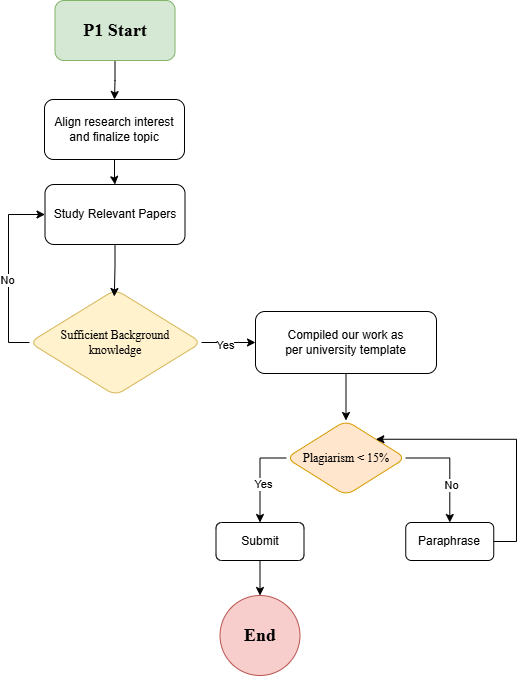
\includegraphics[width=0.6\linewidth]{images/p1_breakdown_1.drawio.png}
    \caption{Workflow of Pre-thesis 01}
    \label{fig:Workflow of Pre-thesis 01}
\end{figure}



\subsection{Tentative Breakdown of Pre-Thesis 2}

Our initial research plan involves proposing a lightweight and domain-specific Retrieval-Augmented Generation (RAG) framework optimized for the legal domain in Bangladesh. The following tasks are planned for Pre-Thesis 2:

\begin{itemize}
    \item Collect and preprocess legal datasets (e.g., laws, verdicts, regulations) relevant to the Bangladeshi legal system.
    \item Implement a basic legal document retriever using both traditional and neural retrieval methods.
    \item Fine-tune or adapt a medium or small-sized LLM to the legal domain and evaluate it using standard NLP metrics such as Accuracy, F1-score, BLEU, and ROUGE.
    \item Integrate the retriever and generator to build an initial RAG pipeline.
    \item Conduct qualitative and quantitative evaluations to identify limitations.
    \item Generate a baseline report focusing on generation quality, latency, and legal accuracy.
\end{itemize}

\begin{figure}[H]
    \centering
    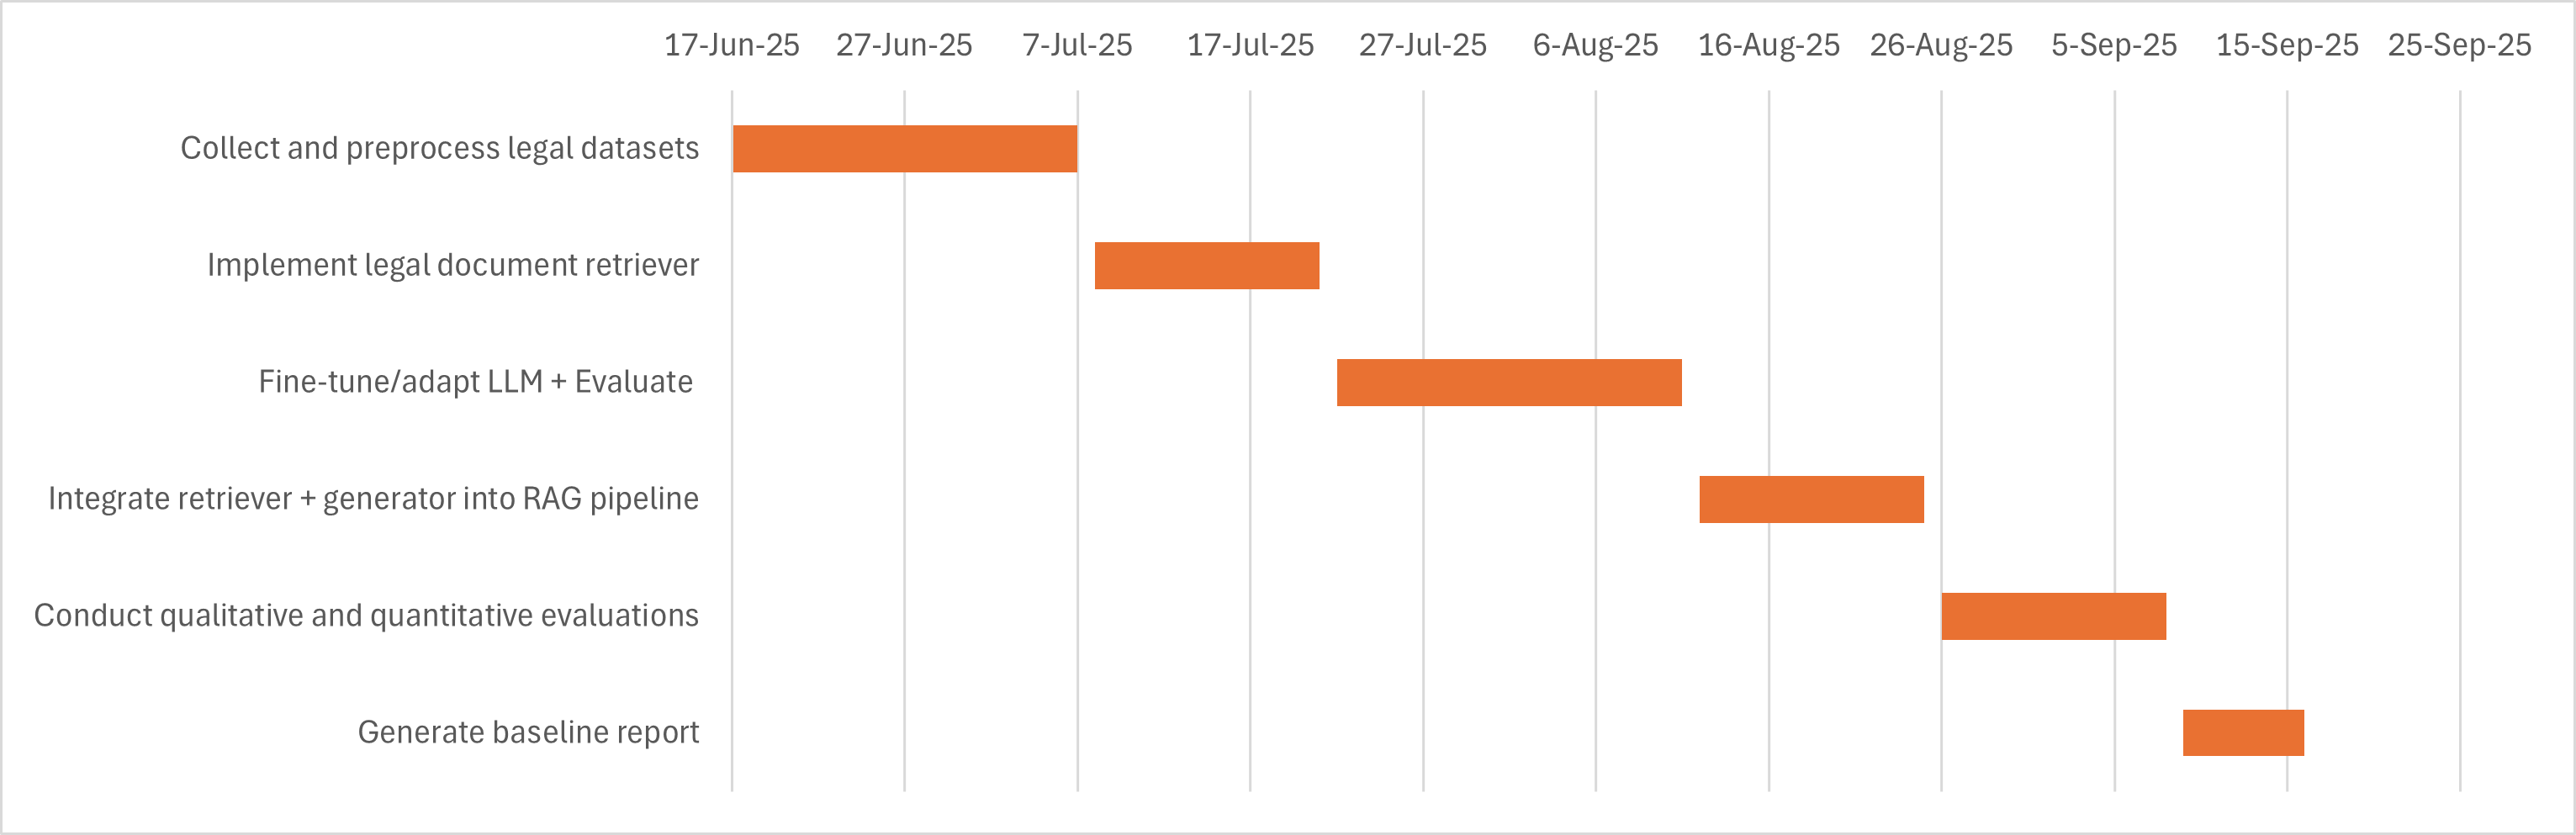
\includegraphics[width=1.0\linewidth]{images/Gantt Chart.png}
    \caption{Gantt chart illustrating the project workflow}
    \label{fig:Gantt chart illustrating the project workflow}
\end{figure}
\subsection{Thesis Defense}

For the final defense, we plan to finalize the distilled and optimized RAG pipeline for legal information access. The tasks to be completed include:

\begin{itemize}
    \item Finalize and evaluate the optimized legal RAG framework.
    \item Prepare a detailed technical report and comprehensive documentation.
    \item Analyze the strengths, weaknesses, and real-world applicability of the system.
    \item Write and submit a research paper summarizing methodology, experiments, and results.
    \item Open-source the project with clean documentation to encourage community involvement and further development.
    \item Identify and submit the work to a suitable peer-reviewed journal or conference in the fields of AI, NLP, or LegalTech.
\end{itemize}


\section{Economic Analysis}


The economic viability of the proposed system involves both development and potential deployment costs. As the system is designed to be resource-efficient and accessible, cost-effective development strategies have been prioritized.

\begin{itemize}
    \item \textbf{GPU Resources:} The majority of model training and experimentation will be conducted using:
    \begin{itemize}
        \item Google Colab Pro: Approx.\ \$10/month for access to T4 or P100 GPUs.
        \item Google Colab Pro+: Approx.\ \$50/month for A100 GPUs and extended runtimes.
        \item Kaggle Kernels: Free GPU access for light preprocessing and testing.
    \end{itemize}
    
    \item \textbf{Software Tools:} All core libraries and frameworks (e.g., PyTorch, Transformers, FAISS, NLTK, SpaCy) are open-source, thus incurring no direct licensing cost.

    \item \textbf{Data Acquisition:} All legal documents are sourced from publicly available government or institutional portals, minimizing data procurement costs.

    \item \textbf{Deployment Costs:} 
    \begin{itemize}
        \item Edge deployment using ONNX or TensorFlow Lite involves no licensing fee.
        \item Mobile front-end development with Flutter or React Native is open-source and free to use.
    \end{itemize}

    \item \textbf{Maintenance and Scalability:} Future maintenance and updates may require continued access to GPU resources and developer time. Community-based open-source collaboration could help reduce long-term costs.

\end{itemize}

Overall, the proposed solution is designed to be cost-effective, with major recurring expenses limited to training compute time on cloud GPU platforms during development phases.



\chapter{Proposed Methodology}
\section{Design Process or Methodology Overview }
Prepare design process based on objectives and constraints.
\section{Preliminary Design or Design (Model) Specification}

Present multiple alternative solutions and perform simulations for verification.

\section{Data Collection -(If
Applicable)}
Sources of data and methods of collection.

\subsection{Data Cleaning}
Techniques used to handle missing values, outliers, and inconsistencies.

\subsection{Data Transformation}
Methods of normalizing, scaling, or encoding data.

\subsection{Data Integration}
Combining data from different sources if applicable.
\subsection{Data Reduction }
Techniques for reducing dimensionality or selecting relevant features.
\subsection{Summary of Preprocessed Data}
Description of the final dataset used for analysis and design.

\section{Implementation of Selected Design}
Describe the implementation process.

\chapter{Result Analysis}
\section{Performance Evaluation}
This section discusses \textbf{evaluation criteria:} key metrics or criteria -accuracy, efficiency, reliability, \textbf{Testing Methods}
\section{Analysis of Design Solutions}
Description of solutions, evaluation criteria - accuracy, efficiency, feasibility, cost, performance, strengths and weaknesses.
\section{Final Design Adjustments}
Make necessary adjustments to the design based on performance evaluation.

\section{Statistical Analysis}

Mention the specific statistical tests or techniques applied

\section{Comparisons and Relationships}

In this section, compare different approaches, compare with existing works, solutions, or results, and analyze their relative effectiveness.


\section{Discussions}
Write about the interpretation, implications, and limitations of the results.






\chapter{Conclusion}
\section{Summary of Findings}
In our study, we point out the revolutionary potential of AI in the legal sphere, specifically, in the sphere of increasing efficiency of such tasks as research and document writing. But also, we identified that the existing Large Language Models (LLM) frequently fail to deal with legal intricacies and can generate misleading counterfeits, or false information, which hamper reliability. This was mitigated by the use of the Retrieval-Augmented Generation (RAG), which essentially meant minimized hallucinations by putting the answers in the perspective of real-life and current knowledge of the law. Although RAG tends to work reasonably well, specific adaptation to complicated multilingual legal environments is necessary since general RAG systems, in this case, can lack required domain knowledge. Our report was able to highlight explicitly the peculiarities of the landscape of the Bangladeshi legal system including the lack of digital sources, uneven access to the internet, and the denominal character of legal documents. To address these, we stress that it requires an intelligent, offline friendly legal AI system with techniques such as Context Awareness Gate (CAG) and  Bangla Natural Language Processing (NLP) that have the ability to negate unnecessary information. More than that, to support the deployment of mobile devices that are prevalent and have resource constraints, model compression algorithms, such as Knowledge Distillation (KD) and Quantization, are needed to decrease the model size and energy cost without compromising accuracy. Lastly, our findings support the idea that, despite the progress being made in multilingual LLMs, building specific Bengali models is essential to resolve the issue, such as the limited availability of data and ineffective text-processors, and make the legal AI solutions practical and effective in Bangladesh.

\section{Contributions to the Field}
Our work contributes both to the advancement of Natural Language Processing (NLP) and the broader societal application of AI technologies. Throughout our research we aimed to address the challenge of making large language models more efficient and accessible, particularly for use in specialized and sensitive domains like legal systems. We tried to show how a large model can be distilled to significantly reduce its size and resource requirement and still preserve its relevancy with the aid of Retrieval Augmented Generation (RAG). This is especially relevant for environments where access to powerful hardware or constant internet connectivity is limited. Additionally, aside from Bangladesh's legal domain, the work contributes to exploring the capabilities of domain-specific data and retrieval strategies can be used to work on edge devices in a decentralized manner preserving user privacy in a local language that remains underrepresented in mainstream research. 
\section{Recommendations for Future Work}
Few existing efforts address the combined challenges of making a small, reliable, interpretable and useful model that can be used offline in a local language on edge devices. Firstly, many legal systems suffer from fragmented, poorly digitized and unstructured legal documents so creating better datasets is essential. Secondly, this research focuses on offline deployment, however the next step should be to investigate how such systems can update securely and ethically preserving user privacy whenever connectivity is available. Thirdly, there is a lack of meaningful benchmark standards in legal NLP. Existing metrics like BLEU or ROUGE are not sufficient for tasks requiring legal precision or domain understanding so a domain specific benchmark involving legal professionals will be crucial. Lastly, these techniques used here should not be limited to law, the same principles can be applied to fields like healthcare, education and public policy which demands access to accurate, interpretable information with low computational requirements.
\phantomsection
\printbibliography % Where the bibliography will be printed
\addcontentsline{toc}{chapter}{Bibliography}

% ********************************** Appendices ********************************
%\begin{appendices} % Using appendices environment for more functionality
\newpage
\phantomsection
\addcontentsline{toc}{chapter}{Appendix A How to install \LaTeX}
\input{appendix/appendix_1}

\newpage
\phantomsection
\addcontentsline{toc}{chapter}{Appendix B Overleaf: GitHub for \LaTeX\ projects}
\input{appendix/appendix_2}
%\end{appendices}

\end{document}